% !TeX spellcheck = en_US
\chapter{Probabilities}
\label{cha:probabilities}

Many \ac{ML} algorithms and problems concern with the \ac{prob} or \ac{pdf} of the outputs from complex inputs. We all aware of some basic examples of the output \ac{prob} from simple inputs, \eg, flipping a coin, rolling a dice. With these simple inputs, due to uncertainty, one could only say about the \ac{prob} that the output could be, \eg, flipping a coin has 50\% of getting head, 50\% of getting tail. Comparing to flipping a coin, inputs for \ac{ML} algorithms are usually more complex, in higher dimensions, in different modals, \etc. The inputs can be datasets, images, audio, \etc. However, as with the simple inputs, we concern ourselves with the \ac{prob} of the outputs, \eg:
\begin{itemize}
	\item Given a dog image, output the \ac{prob} of the breed of the dog.
	\item Image segmentation: given an image, output the \ac{prob} of object class for each pixel.
	\item Cancer detection: given a medical image, output the \ac{prob} of the patient having cancer.
\end{itemize}
This chapter presents important \ac{prob} problems relating to \ac{ML}. For mathematics foundation on \ac{prob}, check the mathematics notes.

\todo{Add image: image with \ac{prob} of being cat or dog}

\section{Parameter Estimation}
Many of \ac{ML} problems are boiled down to finding \textit{statistical models}. Those models predict the \ac{prob} of the data belongs to one class (in classification problem), \ac{prob} of events that will happen, \etc. It all end up with finding a suitable set of \ac{param} for these \textit{statistical models}.

\subsection{Maximum Likelihood Estimation}
\label{subsec:mle}
\ac{MLE} finds the parameters that maximize the \ac{prob} of the existing data.
\begin{align}
	&\text{Model parameter $\theta$:} &&\theta = \underset{\theta}{\arg\max}\:p(x_1, x_2, \dots, x_N | \theta) \\
	&\text{Assuming independent variables:} &&\theta = \underset{\theta}{\arg\max} \prod^N_{n=1} p(x_n | \theta) \\
	&\text{Maximum log-likelihood:} &&\theta = \underset{\theta}{\arg\max} \sum^N_{n=1} \left[\text{log}\:p(x_n | \theta) \right]\\
	&\text{Minimum negative log-likelihood:} && \theta = \underset{\theta}{\arg\min} \sum^N_{n=1} \left[-\text{log}\:p(x_n | \theta)\right]
\end{align}

\subsection{Maximum A Posteriori}
Sometimes, prior knowledge of the \ac{pdf} is presented. \Eg, the \ac{prob} of getting head when flipping a coin is around 50\%. \ac{MAP} takes advantage of the prior knowledge $p(\theta)$ on the parameters $\theta$ by applying Bayes rule.
\begin{equation}
	\theta = \underset{\theta}{\arg\max} \prod^N_{n=1} p(x_n | \theta)p(\theta)
\end{equation}
\hlr{\ac{MLE} (\secref{subsec:mle}) suffers when there is not enough data} $\Rightarrow$ \hlr{use \ac{MAP}}

\section{Naive Bayes Classifier}
The word \textit{naive} implies having the independence assumption on the variables.
\begin{align}
	c 	&= \underset{c \in \mathbb{C}}{\arg\max}\ p(c|x)\\
		&= \underset{c \in \mathbb{C}}{\arg\max}\ p(x|c)\,p(c)
\end{align}

If $x$ is:
\begin{itemize}
	\item continuous variable $\Rightarrow$ Gaussian Naive Bayes
	\item feature vector $\Rightarrow$ Multinomial Naive Bayes
	\item binary vector $\Rightarrow$ Bernoulli Naive Bayes
\end{itemize}

Minimize the expected loss: $\displaystyle \expectation{L} = \sum_{k}\sum_{j}\int_{R_j}L_{kj}\,p(x, C_k)\,dx$ by choosing region $R_j$ such that $\displaystyle \expectation{L} = \sum_kL_{kj}\,p(C_k| x)$

\section{Views on the Decision Problem}
\subsection{Generative Methods}
First determine the class-conditional densities and separately infer the prior class \ac{prob} $\Rightarrow$ Bayes theorem $\Rightarrow$ class membership
\[p(x|C_k)\,p(C_k) \Rightarrow y_k(x)\]
\Eg, Mixture of Gaussians

\subsection{Discriminative Methods}
First solve the inference problem of determined the posterior class \ac{prob}

\subsection{Classification with Loss Functions}
For classification problem with more than 2 classes, the output's predicted class $\mathcal{C}_k$ is the one with the greatest posterior \ac{prob} among all classes $\mathcal{C}_j$, which can still be wrong:
\begin{align*}
	p(\mathcal{C}_k|x) &> p(\mathcal{C}_j|x) && \forall j \neq k && && \\
	p(x|\mathcal{C}_k)p(\mathcal{C}_k) &> p(x|\mathcal{C}_j)p(\mathcal{C}_j) && \forall j \neq k && &&
\end{align*}
Loss function differentiate the possible decisions and the possible true classes. \Eg:
\begin{itemize}
	\item Decisions: \textit{sick} or \textit{healthy}
	\item Classes: patient is \textit{sick} or \textit{healthy}
\end{itemize}
The cost may be symmetric. In this case however, it is asymmetric:
\[\text{\textit{loss(decision=healthy | patient=sick)}} >> \text{\textit{loss(decision=sick | patient=healthy)}} \]
The classification problem could be formalized by introducing loss matrix $L_{kj}$
\[ L_{kj} =$ \textit{loss for decision} $\mathcal{C}_j$ \textit{if truth is} $\mathcal{C}_k \]
\Eg, cancer diagnosis:
\[L_{cancer\;diagnosis} = \begin{matrix}
	  & & \textbf{Decision}\\
	  & & \begin{matrix}
	  		cancer & normal
	  \end{matrix}\\
  	\textbf{Truth} & \begin{matrix}
  		cancer \\ normal
  	\end{matrix} & \begin{pmatrix}
		0 & 1000\\
		1 & 0
	\end{pmatrix}
\end{matrix}\]
Loss functions maybe different for different actors:
\[ L_{stocktrader}(subprime) \neq L_{bank}(subprime)\]

\subsection{Minimize the Expected Loss}
But regardless, the optimal solution is the one that minimizes the \textit{expected loss}. It is \textit{expected} loss because it depends on the true class, which is unknown.\\
$\Rightarrow$ \hlb{Minimize the expected loss}

\Eg, 2 class $C_1, \; C_2$, 2 decisions $\alpha_1, \; \alpha_2$.

The loss: $L(\alpha_j | C_k) = L_{kj}$.

The expected loss is equal to the risk $R$.
\begin{align*}
	\mathbb{E}_{\alpha_1}[L] = R(\alpha_1|x) = L_{11}\,p(C_1|x) + L_{21}\,p(C_2|x)\\
	\mathbb{E}_{\alpha_2}[L] = R(\alpha_2|x) = L_{12}\,p(C_1|x) + L_{22}\,p(C_2|x)\\
\end{align*}
Choose $\alpha_1$ if $R(\alpha_1|x) < R(\alpha_2|x)$

% !TeX spellcheck = en_US

\section{Probability Density Estimation}
\label{cha:pdf-estimation}
The following approaches' aim is to estimate an unknown \ac{pdf}.
\begin{itemize}
	\item \hlb{Non-parametric approaches:} represent the \ac{pdf} without parameter, usually as a lookup table. Using lookup table is fast, but could also be memory-consuming.\\
	Among the presented ones, only histogram is non-parametric.
	\item \hlb{Parametric approaches:} within sufficiently small region $\mathcal{R}$, the \ac{prob} can be estimated as $\displaystyle p = \int_{\mathcal{R}}p(y)dy \approx p(x)V = \frac{K}{N.V}$, where $K$ is the number of data points in the region, $V$ is the volume of the region.
\end{itemize}

\subsection{Histogram}
The \ac{prob} of a bin:
\begin{equation}
	p_i = \frac{n_i}{N.\Delta_i}
\end{equation}

in which $n_i$ is the number of data points in that bin, $N$ is the total number of data point, $\Delta_i$ is the width of the bin, often $\Delta_i=\Delta$.

\hlb{Notes}:
\begin{itemize}
	\item $\Delta$ serves as the \hlr{smoothing factor}
	\item With $D$ as the dimensions of the data points. The number of bins grow exponentially with $\mathcal{O}(k^D)$
\end{itemize}
\begin{figure}[hbt!]
	\centering
	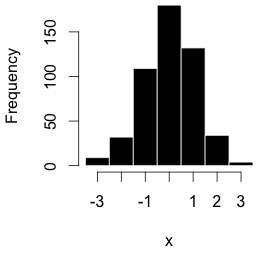
\includegraphics[width=0.25\textwidth]{histogram.png}
	\caption{Example of a histogram, $\Delta = 1$ (\href{https://en.wikipedia.org/wiki/Histogram}{src}).}
\end{figure}

\subsection{Kernel Methods}
The kernel methods fix the volume $V$ and determine the number of data points $K$. The volume $V$ is the space restricted within a parzen window $k(u)$ that satisfies $k(u) \geq 0$.
\begin{align}
	&\text{A hyper-space cube:} && k(u) = \begin{cases}
		1\;\; if \;\; |u_i| \leq \frac{1}{2}h, \;\; i = 1, 2, \dots, D \\
		0\;\; else
	\end{cases} \\
	&\text{The number of points inside:} &&K = \sum_{n=1}^{N} k(x-x_n) \\
	&\text{The region \textit{volume}:} &&V = \int k(u) du = h^D\\
	&\text{The probability:} && \Rightarrow p(x) \approx \frac{K}{N.V} = \frac{1}{N.h^D}\sum_{n=1}^{N}k(x-x_n)
\end{align}
\note the above parzen window is asymmetric.\\
The \hlb{symmetric Gaussian kernel is a better substitution}.
\begin{align}
	&\text{A Gaussian kernel:} && k(u) = \frac{1}{\sqrt{2\pi h^2}}\:exp\left(\frac{-u^2}{2h^2}\right) \\
	&\text{The region \textit{volume}:} &&V = \int k(u) du = 1 \\
	&\text{The probability:} && \Rightarrow p(x) \approx \frac{1}{N} \sum_{n=1}^{N} \frac{1}{(2\pi)^{D/2}h}\:exp\left(\frac{-||x-x_n||^2}{2h^2}\right)
\end{align}
For Kernel methods, $h$ is the \hlb{smoothing factor}.

Generalization: $k(u) \geq 0$, $\displaystyle \int k(u)du = 1$.

\hlr{Size of the hypersphere is proportional to $h^2$.}

\subsection{K-Nearest Neighbor}
When you fix the number of data points $K$ and determine the volume $V$, it leads to K-Nearest Neighbor.
\begin{figure}[!hbt]
	\centering
	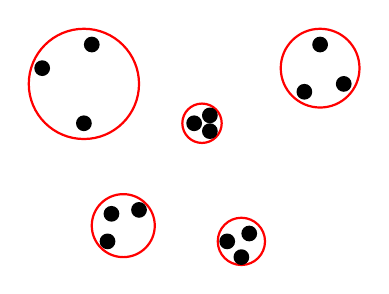
\begin{tikzpicture}
		\draw[red,thick](1,3) circle (.7);
		\fill[black] (.47,3.2) circle (0.1);
		\fill[black] (1.1,3.5) circle (0.1);
		\fill[black] (1,2.5) circle (0.1);
		\draw[red,thick](4,3.2) circle (.5);
		\fill[black] (4.3,3) circle (0.1);
		\fill[black] (4,3.5) circle (0.1);
		\fill[black] (3.8,2.9) circle (0.1);
		\draw[red,thick](2.5,2.5) circle (0.25);
		\fill[black] (2.6,2.6) circle (0.1);
		\fill[black] (2.6,2.4) circle (0.1);
		\fill[black] (2.4,2.5) circle (0.1);
		\draw[red,thick](1.5,1.2) circle (0.4);
		\fill[black] (1.7,1.4) circle (0.1);
		\fill[black] (1.3,1) circle (0.1);
		\fill[black] (1.35,1.35) circle (0.1);
		\draw[red,thick](3,1) circle (0.3);
		\fill[black] (3.1,1.1) circle (0.1);
		\fill[black] (2.82,1) circle (0.1);
		\fill[black] (3,.8) circle (0.1);
	\end{tikzpicture}
	\caption{K-Nearest Neighbor with $K=3$.}
\end{figure}

\begin{equation}
	p(x) \approx \frac{K}{NV}
\end{equation}
Here, $K$ is the \hlb{smoothing factor}.

\hlr{\begin{itemize}
		\item Too much bias $\Rightarrow$ too smooth
		\item Too much variance $\Rightarrow$ \underline{NOT} smooth enough
	\end{itemize}
	$\Rightarrow$ combine parametric methods to a mixture model}

\hlr{Mixture distribution = multi-parametric model}

\subsection{Mixture of Gaussians}
\ac{MoG}, as \hlr{Generative Model}, is defined from the sum \ac{prob} of elemental Gaussians: $\displaystyle p(x|\theta) = \sum_{j=1}^{M}p(x|\theta_j)p(j)$, where $p(x|\theta_j)$ is a \hlr{mixture component}, $p(j) = \pi_j$ is the \hlr{weight of the component}
\begin{align}
	p(x|\theta_j) &= \frac{1}{\sqrt{2\pi}\sigma_j}\:\exp\left[\frac{-(x-\mu_j)^2}{2\sigma_j^2}\right],\;\;p(j)=\pi_j, \;\;\sum\pi_j=1 \\
	p(x|\theta_j) &= \frac{1}{(2\pi)^{\frac{D}{2}}|\Sigma_j|^{\frac{1}{2}}}\:\exp\left[-\frac{1}{2}(x-\mu_j)^T\Sigma_j^{-1}(x-\mu_j)\right]
\end{align}

\subsection{K-Means Clustering}
There are 3 steps. Step 2 and 3 are repeated until there is no change.
\begin{enumerate}
	\item Pick $K$ centroids
	\item Assign sample to the centroid
	\item Adjust centroids
\end{enumerate}
\note Check \href{https://machinelearningcoban.com/2017/01/01/kmeans/}{machinelearningcoban.com}.
\begin{itemize}
	\item This leads to a local optimum, depends on initialization.
	\item It's sensitive to \hlb{outliers}, detects \hlb{spherical clusters only}.
	\item Application: \eg, image compression.
\end{itemize}

\subsection{EM Clustering}
Assuming $N$ data points and $K$ Gaussians.
\begin{itemize}
	\item \textbf{E-Step:} Fix the Gaussians, find $\gamma_j(x)$, which represent the \hlr{responsibility of component $j$ for data point $x$}.
	\begin{equation}
		\gamma_j(x_n) = \frac{\pi_j \mathcal{N}\left(x_n|\mu_j,\Sigma_j\right)}
		{\sum_{k=1}^{K}\pi_k \mathcal{N}\left(x_n|\mu_k,\Sigma_k\right)} \tab \forall j=1, 2, \dots, K, \;\; n=1, 2, \dots, N
	\end{equation}	
	\item \textbf{M-Step:} Fix $\gamma_j(x)$, update the Gaussians.
	\begin{align}
		\hat{N}_j &= \sum_{n=1}^{N}\gamma_j(x_n) \\
		\hat{\mu}_j &= \frac{1}{\hat{N}_j} \sum_{n=1}^{N} \gamma_j(x_n)x_n \\
		\hat{\pi}_j &= \frac{\hat{N}_j}{N} \\
		\hat{\Sigma}_j &= \frac{1}{\hat{N}_j} \sum_{n=1}^{N} \gamma_j(x_n) \left(x_n - \hat{\mu}_j\right)\left(x_n - \hat{\mu}_j\right)^T
	\end{align}
\end{itemize}
\hlb{Notes}:
\begin{itemize}
	\item EM is short for Expectation-Maximization
	\item Regularization with $\Sigma + \sigma_{min}I$
	\item Initialization $\mu_j$ with K-Means
	\item Compare with K-Means
	\begin{itemize}
		\item Hard-assignment $\Leftrightarrow$ K-Means: each data point to 1 class
		\item Soft-assignment $\Leftrightarrow$ EM Clustering: each data point $\Rightarrow$ \ac{prob} to fall into many classes
		\item With \hlr{more \ac{param}}, EM \hlr{needs more iteration}.
	\end{itemize}	
\end{itemize}